\chapter{Systembechreibung}

\section{Lösungsstrategie}

\subsection{Templates}


\subsection{Controller}

\subsection{Producer}

\subsection{ServiceBeans}

\subsection{JPA}





Die Grundidee hinter dem Framework basiert auf dem Gedanken, dass alle simplen \acs{CRUD}-Anwendungen ein gleiches Verhalten aufweisen, da sie die selbe Funktionalität
zur Verfügung stellen, nämlich \textit{Lesen, Schreiben, Löschen und Ändern}.
Wenn man eine weitestgehend individuelle Benutzeroberfläche außer Acht lässt, liegt der einzige Unterschied zwischen den Anwendungen im Inhalt und der Bedeutung der Datenmodelle.
Darauf basierend braucht es auch an das Datenmodel angepasste Darstellungen in der Benutzeroberfläche.
Das CRUD-Framework geht davon aus, dass ein Datenmodel einer \acs{CRUD}-Anwendung aus drei Komponenttypen besteht. 
Die \enquote{Viewable}-Komponenten, die im Normalfall den Klassen des Datenmodels und den JPA-Entities. 
Die \enquote{ModelLists}, die Sammlungen von Viewable-Komponenten darstellen. 
Die \enquote{Associations}, die eine Erweiterung der ModelList sind. Sie bilden die Beziehungen zwischen den einzelnen Datenmodel-Elementen.\\
\\
Diese abstrakte Darsellung der Datenmodel-Elemente ist ausreichend um die gesamte Funktionalität einer CRUD-Anwendung abbilden zu
können. Diese Eigenschaft macht sich das \acs{CRUD}-Framework zu nutze. Ein Anwender muss nur noch die definierte Schnittstelle in sein Datenmodel implementieren und 
passende XHTML-Temlates für die Darstellung der Elemente erstellen.

\section{Anforderungen}

Das Framework muss in der Lage sein ein Datenmodell und dazugehörige Templates im XTHML Format entgegen zunehmen und eine funktionierende
CRUD-Applikation daraus zu machen. Das Framework soll die gesamte Steuerung der Applikation übernehmen, indem es eine
Reihe von Steuereinheiten und Interfaces zur Verfügung stellt. Einer der Hauptansprüche des Systems, ist eine
automatische Erkennung der Relationen zwischen den Datenmodellen und die richtige Abbildung derer.
Desweiteren sind Hauptanforderungen an das Framework eine Schnittstelle für Fehlermeldungen und Logging. 
Die Daten werden vom System mittels JPA persistiert, sofern das Datenmodell JPA-Entitäten implementiert.

\section{Datenmodel des Frameworks}

In den vorhergehenden Kapiteln wurden das Datenmodel des Frameworks bereits erläutert. Die Datenstruktur ist in der Abbildung
\ref{pic:guimodel} dargesstelt. Dieses besteht aus drei Elementen:\\



\begin{figure}[htb!]
	\caption{GUI-Modell Klassendiagramm}
	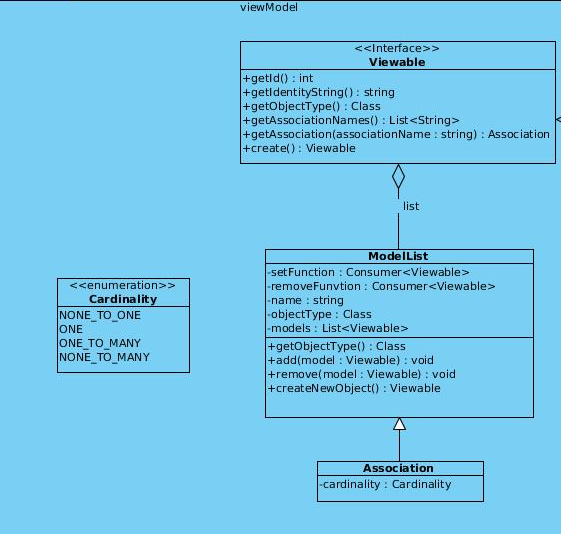
\includegraphics[width=0.9\textwidth]{content/pictures/Guimodel}
	\label{pic:guimodel}
\end{figure}

\section{Templates}
Als Templates werden die XHTML-Vorlagen bezeichnet. Diese können in zwei Gruppen aufgeteil werden: Object-Templats und Service-Templates.
Die Object-Templates werden für die Darstellung der einzelnen Viewable-Objekte verwendet. Diese müssen einem bestimmten Namenschema folgen, welches
den Klassenname beinhaltet. Der Inhalt der Objekt-Templates kann abhängig vom Anwendungsfall angepasst werden. Die einzelnen Elemente 
dieser Templates können zusätliche Validierungskriterien beinhalten.\\
\\
Die Templates sind durch Kompositionen miteinander verknüpft. 
Die Applikation beginnt in der Hauptansicht dem Index-Template, von welcher man in vier Listenansichten gelangt. In einer Listenansicht, 
kann man ein neues Objekt erzeugen, ein vorhandenes Objekt bearbeiten bzw. löschen, oder einfach einsehen. Wenn man ein Objekt löscht, so bleibt man in der Listenansicht - 
In jedem anderen Fall gelangt, man in die Objektansicht.
Jede Objektansicht besitzt Referenzen auf andere Objekte, also Assoziationen. Diese Referenzen, werden in der Objektansicht ebenfalls 
gezeigt. Wenn man diese Referenz einsehen will, so gelangt man immer zunächst in die Listenansicht der angeforderten Objekte, 
auch wenn nur ein Objekt vorhanden ist.
\\
Die Service-Templates verwenden nur die Objekte der \enquote{AbstractModel}-Komponente und können nach Bedarf Object-Templates einbinden.
Es gibt folgende Service-Templates:\\
\begin{description}
\item[Index-Template] 
Ist das Template für die Hauptseite der Benutzeroberfläche. Es beinhaltet die \enquote{Sidebar} der Anwendung. Zusätzlich enthält es das \enquote{Contentpane} der Anwendung, in dem andere 
Templates eingefügt werden können. In Abbildung \ref{pic:semVer_allViews} sieht man eine Repräsentation der Hauptansicht der integrierten Listenansicht und einer Objektansicht.
\item[ListView]
Ist das Template für die Listenansichten. Es wird für die Darstellung der ModelList bzw. Association verwendet. Eine ListView beinhaltet immer zugehörige Object-Templates, da
man einzelne Objekte innerhalb der Listenansicht ebenfalls ansehen kann.
\item[NewView]
Das Tempalte wird bei der Ertellug eines neuen Objekts verwendet. Es bindet die zugehörigen Object-Templates sowie das SelectView-Template ein.
\item[SelectView]
Dieses Template wird verwendet wenn existierende Objekte zu einer Assoziation hizugefügt werden sollen. Ein Beispiel sieht man in Abbildung \ref{pic:semVer_selectView}
\item[LogInView]
Ein Template, welches für die Benutzerauthentifizierung verwendet wird. Die dazugehörige Umsetzung sieht man in Abbildung \ref{pic:semVer_loginView}
\end{description}


\begin{figure}[htb!]
	\caption{Templates Screenshot}
	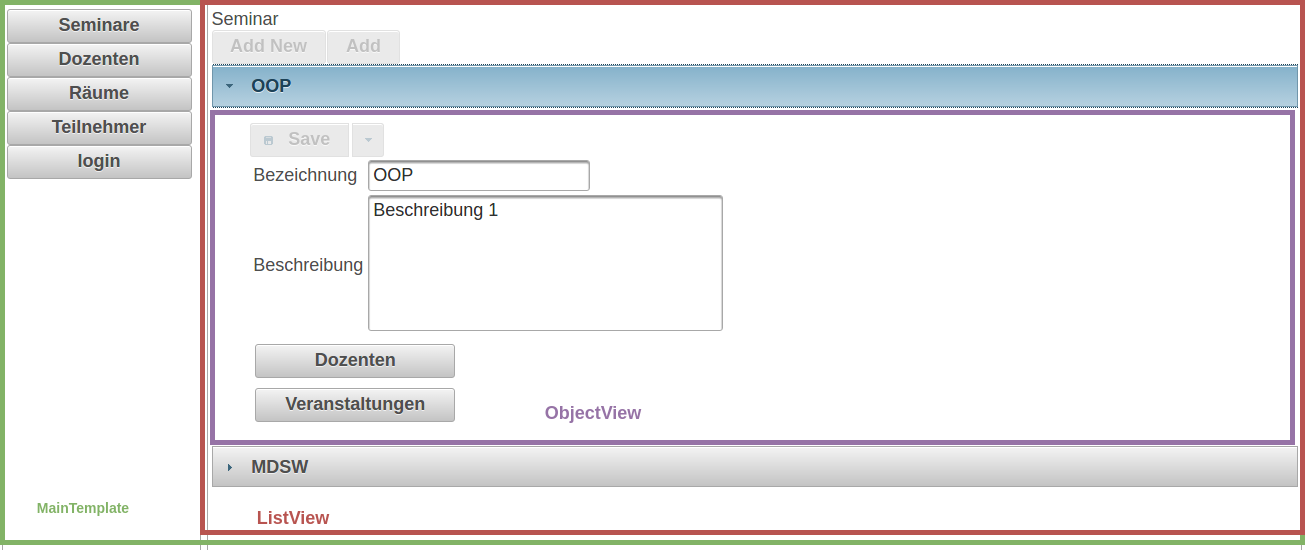
\includegraphics[width=0.9\textwidth]{content/pictures/Seminarverwaltung_ListAndObjectView}
	\label{pic:semVer_allViews}
\end{figure}

\begin{figure}[htb!]
	\caption{LoginView Screenshot}
	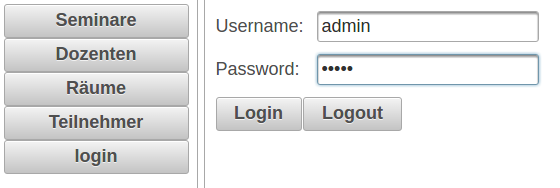
\includegraphics[width=0.9\textwidth]{content/pictures/Seminarverwaltung_LoginView}
	\label{pic:semVer_loginView}
\end{figure}

\begin{figure}[htb!]
	\caption{SelectView Screenshot}
	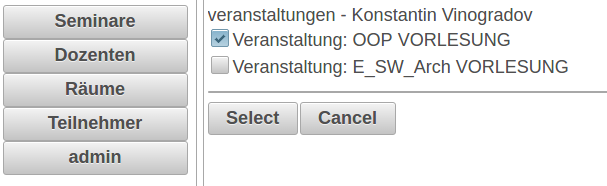
\includegraphics[width=0.9\textwidth]{content/pictures/Seminarverwaltung_SelectView}
	\label{pic:semVer_selectView}
\end{figure}

\newpage

\section{Controller}

Die Controller-Komponenten können, mit der Ausnahme des MainController, in zwei Gruppen aufgeteilt werden: UI- und Service-Controller.
Die UI-Controller sind für die Funktionalität einzelner Ansichten zuständig. Die Serivce-Controller regeln den Datenbankzugriff,
Fehlerbehandlung und Logging.

\subsection{MainController}
Der MainController nimmt eine Sonderrolle ein. Er dient als Kommunikations-Knotenpunkt und bestimmt welcher UI-Controller die Steuerung 
übernehmen soll. Dies ist die Hauptsteuereinheit, weswegen sie alle anderen Steuereinheiten kennt und deligiert. Zusätzlich steuert sie,
welches Template gerade sichtbar ist.

\subsection{UI-Controller}

Diese Steuereinheiten sind rein für die Verwaltung und Kommunikation der Benutzeroberfläche verantwortlich.
Die drei wichtigsten Steuereinheiten sind der \enquote{ListViewController}, \enquote{SelectViewController} und \enquote{NewViewController},
die ausführlicher erläutert werden.

\paragraph{ListViewController}

Der ListViewController ist für die Verwaltung der Listenansicht zuständig. Der MainController überträgt ihm die Kontrolle
nachdem mit dem Loaderkommuniziert wurde, um die benötigten Daten aus der Datenbank zu laden.\\
\\
Der typische Ablauf für diese Steuereinheit ist das Anzeigen einer Liste. 
Der Ablauf bei der Erstellung der Listenansicht ist in dem Diagramm \ref{pic:showListSeq_diag} dargestellt. Dabei bindet 
das ListView-Template zugehörige Objekt-Templates zur Laufzeit ein. Die Datenobjekte und die Information, ob der Nutzer
die Daten bearbeiten darf, werden bei der Anbindung übergeben. Eine Typprüfung der Datenobjekte findet nicht statt.

\begin{figure}[htb!]
	\caption{ShowList Sequenzdiagramm}
	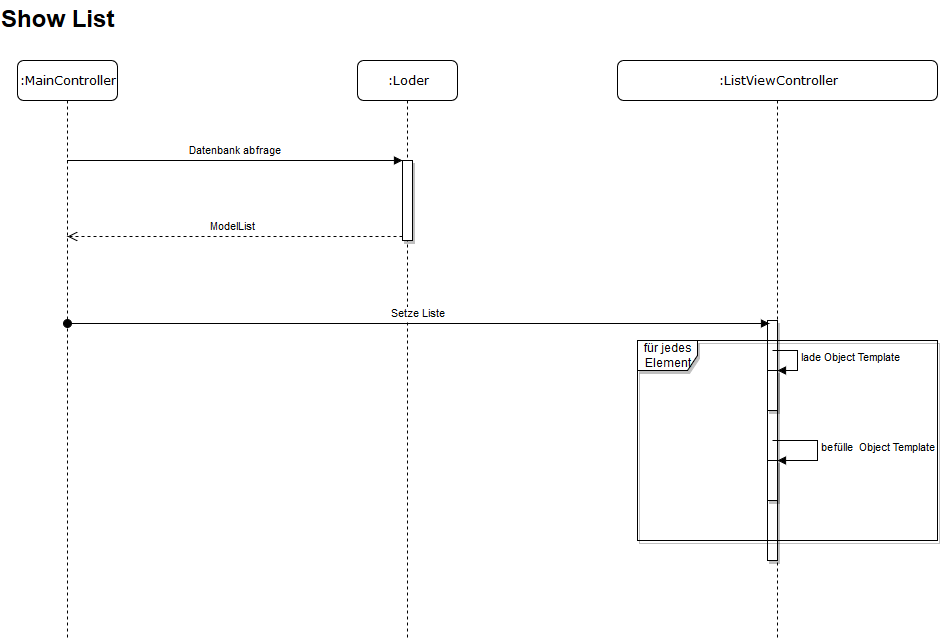
\includegraphics[width=0.9\textwidth]{content/pictures/ShowListSeq}
	\label{pic:showListSeq_diag}
\end{figure}

\paragraph{SelectViewController}
Der SelectViewController ist für die Zuordnung von existierenden Objekten zu anderen Objekten zuständig. Er ermöglicht z.B.,
dass in diesem generischen Ansatz ein Teilnehmer einer Veranstaltung zugeordnet werden kann.\\
\\
Die Select Funktionalität wird von der Listenasicht zur Verfügung gestellt. Sie wird nur für die Assoziationsdarstellung benötigt. 
Der Ablauf ist in dem Diagramm \ref{pic:selectSeq_diag} dargestellt. Zu vermerken ist, dass die Validerung der Auswahl anhand der
Kordinalität seiner Assoziation, nicht unter die Aufgaben des SelectViewControllers fällt.  

\begin{figure}[htb!]
	\caption{Select Sequenzdiagramm}
	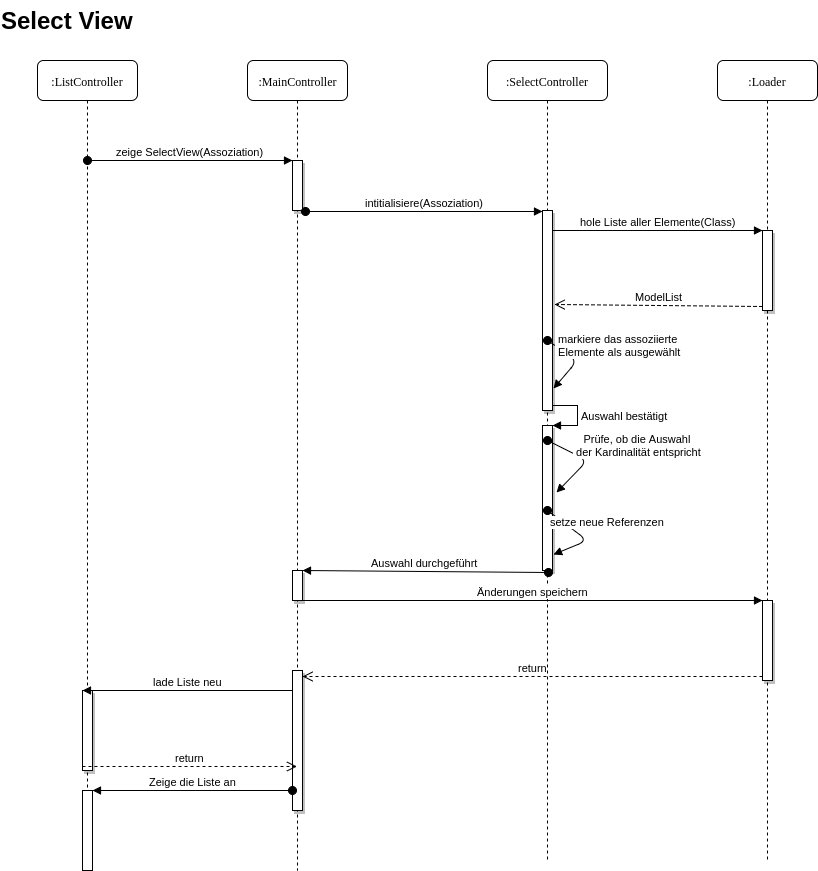
\includegraphics[width=0.9\textwidth]{content/pictures/SelectSeq}
	\label{pic:selectSeq_diag}
\end{figure}



\paragraph{NewViewController}
Der NewViewController ist für die korrekte Erzeugung und Zuordung eines neu angelegten Objektes und seiner Abhängigkeiten verantwortlich.
\\
\\
Das Diagramm \ref{pic:createNewViewSeq_diag} stellt die Kommunikation zwischen den Controller-Elementen bei der Erstellung eines neun
Datenobjekts dar. Der Vorgang kann aus der ListView ausgelöst werden. Der Ablauf unterscheidet sich abhängig davon, ob es sich bei
dem Ausgangselement um eine \enquote{ModelList} oder eine \enquote{Association} handelt. Bei einer Association kann das Datenobjekt automatisch bei der Erstellung gestzt
werden.

\begin{figure}[H]
	\caption{CreateNewView Sequenzdiagramm}
	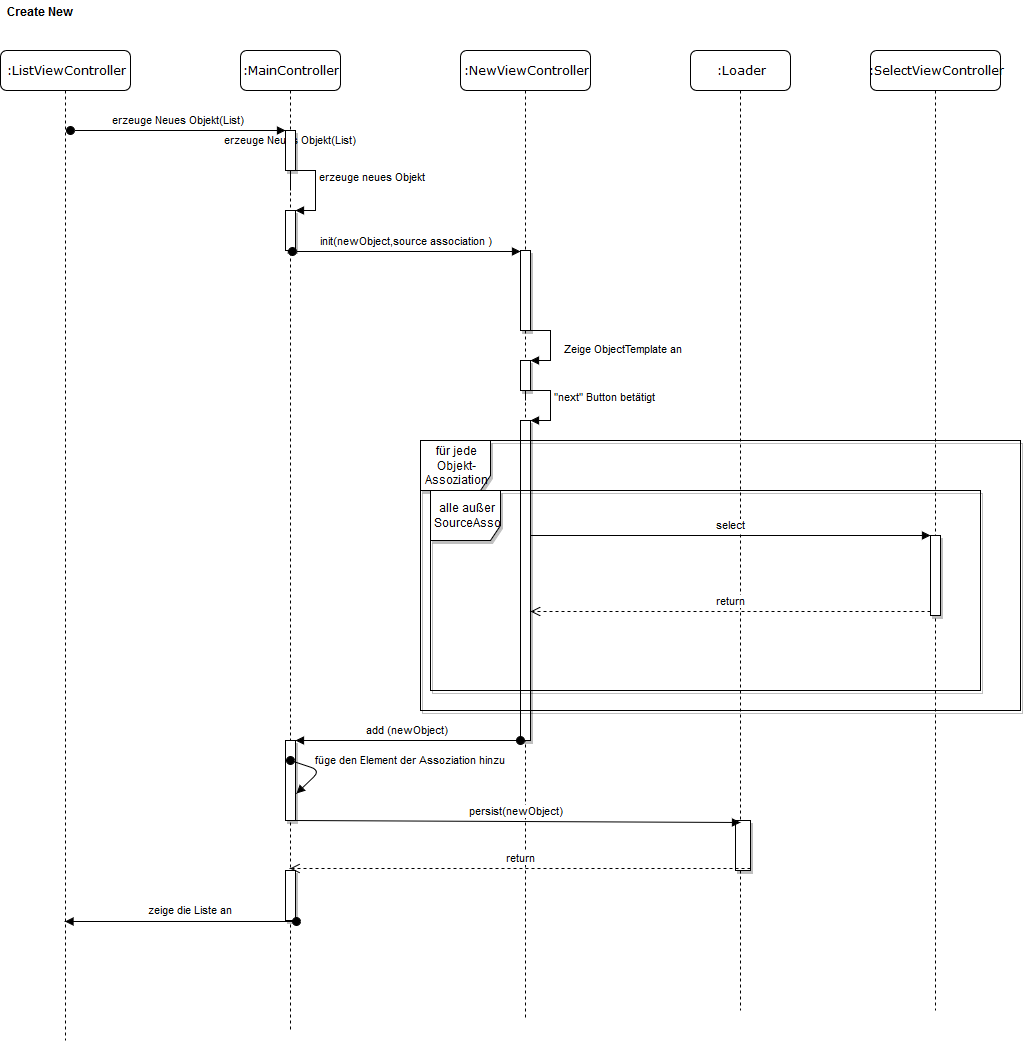
\includegraphics[width=0.9\textwidth]{content/pictures/CreateNewView}
	\label{pic:createNewViewSeq_diag}
\end{figure}

\paragraph{UserLoginController}
Der UserLoginController regelt die Zugriffsrechte im System und ist für den gesamten Login-Vorgang verantwortlich.\\
\\
Wenn ein Benutzer sich am System anmelden will, so gibt er seine Nutzerdaten ein. Diese Steuereinheit sucht nach dem Nutzernamen und
entschlüsselt das AES verschlüsselte Passwort, um es mit der Eingabe abzugleichen. Sollte der Vorgang erfolgreich sein, wird ein
globaler Flag umgeswitcht, welcher die Bearbeitungsfunktionalität freischält.

\subsection{Service-Controller}

Die Service-Controller werden von anderen Controllern verwendet, werden aber nicht direkt aus der UI angesprochen.
Es gibt die folgenden zwei Service-Controller:\\

\paragraph{MessagesViewController}
Der MessagesViewController ist ein Wrapper für unsere Logging-Komponente \enquote{log4J}. Es bietet die Möglichkeit alle Ereignisse
an zentraler Stelle zu verwalten und ermöglicht gleichzeitig die Kommunikation mit dem Nutzer, über diverse Anzeigen, die Primefaces
zur Verfügung stellt.

\paragraph{Loader}

Der Loader übernimmt die Kommunikation mit der Datenbank. Er hält einen EntityManger und \acs{CRUD}-Funktionalität für die Datenbank.
Zusätzlich enthält diese Steuereinheit den Datenbank-Treiber, welcher benötigt wird, da wir uns für eine lokale Datenbank entschieden haben
und \acs{JPA} dann keine automatische Konfiguration vornehmen kann.


